\documentclass{article}

\usepackage{amsmath}
\usepackage{geometry}
\usepackage{graphicx}

\usepackage[utf8]{inputenc}
\usepackage{fourier} 
\usepackage{array}
\usepackage{makecell}

\renewcommand\theadalign{bc}
\renewcommand\theadfont{\bfseries}
\renewcommand\theadgape{\Gape[4pt]}
\renewcommand\cellgape{\Gape[4pt]}

\geometry{letterpaper, left=1cm, right=1cm, top=1.5cm, bottom=2cm}

\title{Adversarial Images}
\author{Adam Spindler}

\begin{document}
\maketitle

\section{Introduction}

Image classification and detection models are commonly used in real world applications such as autonomous vehicles \cite{CGV-079} and intrusion detection \cite{KIM2018845}. It's important that these systems are reliable and robust to attacks as reliance upon them increases. If it is possible to hide signs from an autonomous vehicle the results could be disastrous.

\section{Adversarial Examples by Random Perturbation}

\subsection{Adding Noise}
Noise was added to the images by generating a random tensor the same size as the input image. The random tensor's values are between 0 and 1, and the image's pixel values are between 0 and 255. To adjust the noisiness of the images, the random tensor was multiplied by the integer parameter "noise" to scale it up. The noise multiplier used in each of the images is shown at the top of the column.

\begin{center}
\begin{tabular}{ c c c c }
    original & noise = 100 & noise = 200 & noise = 500 \\
    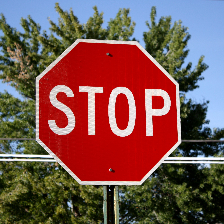
\includegraphics[width=0.2\linewidth]{../test_images/stop.png} & 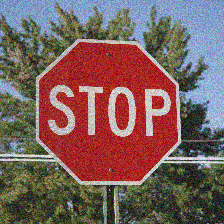
\includegraphics[width=0.2\linewidth]{../test_images/perturbed/stop_noise_100.png} & 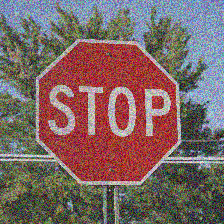
\includegraphics[width=0.2\linewidth]{../test_images/perturbed/stop_noise_200.png} & 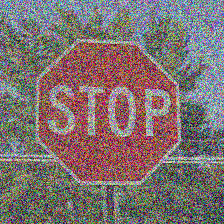
\includegraphics[width=0.2\linewidth]{../test_images/perturbed/stop_noise_500.png} \\
    \makecell{YOLOv3 = 0.99987 \\ RCNN = 0.99987} & \makecell{YOLOv3 = 0.99987 \\ RCNN = 0.99993} & \makecell{YOLOv3 = 0.99968 \\ RCNN = 0.99610} & \makecell{YOLOv3 = 0.99985 \\ RCNN = 0} \\[1cm]
    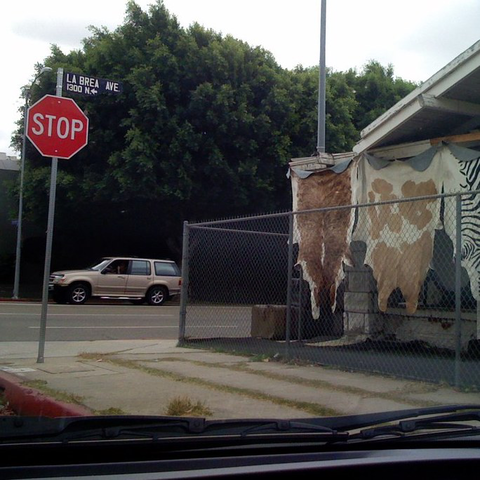
\includegraphics[width=0.2\linewidth]{../test_images/stop3.png} & 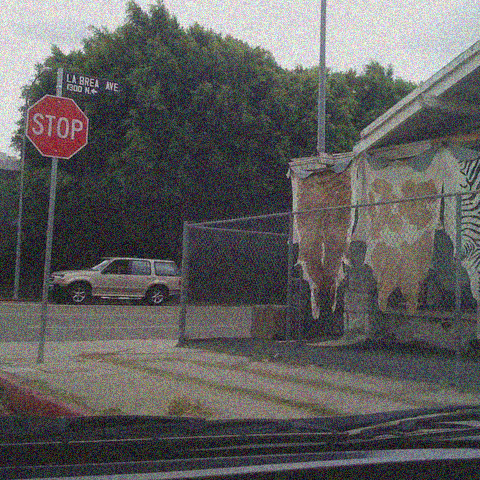
\includegraphics[width=0.2\linewidth]{../test_images/perturbed/stop3_noise_100.png} & 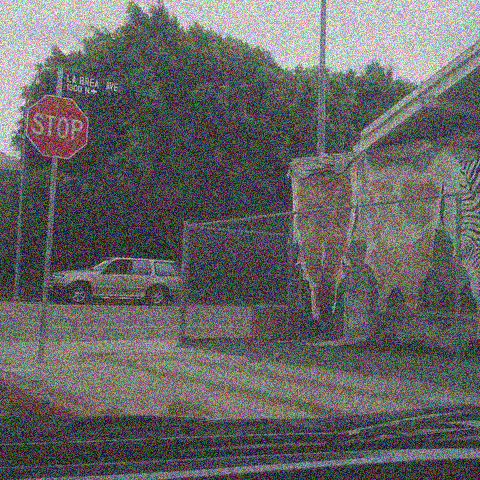
\includegraphics[width=0.2\linewidth]{../test_images/perturbed/stop3_noise_200.png} & 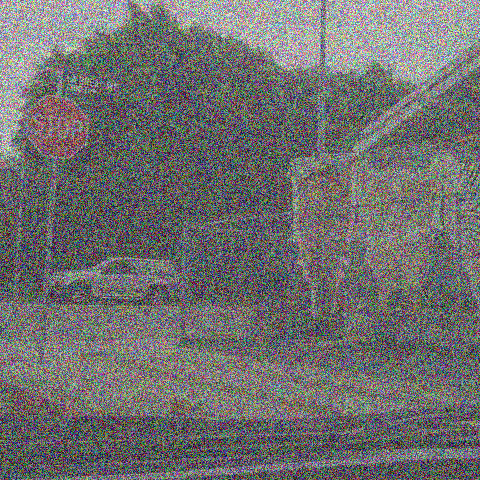
\includegraphics[width=0.2\linewidth]{../test_images/perturbed/stop3_noise_500.png} \\
    \makecell{YOLOv3 = 0.99971 \\ RCNN = 0.99839} & \makecell{YOLOv3 = 0.99995 \\ RCNN = 0.99926} & \makecell{YOLOv3 = 0.99951 \\ RCNN = 0.99850} & \makecell{YOLOv3 = 0 \\ RCNN = 0} \\  
\end{tabular}
\end{center}

\subsection{Grayscale}
The images were converted to grayscale by removing a percentage of their colors. The value used for each of the images is shown at the top of the columns.
\begin{center}
\begin{tabular}{ c c c c }
    original & color = 50\% & color = 25\% & color = 0\% \\
    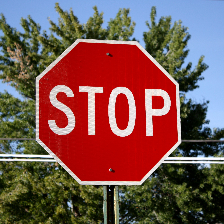
\includegraphics[width=0.2\linewidth]{../test_images/stop.png} & 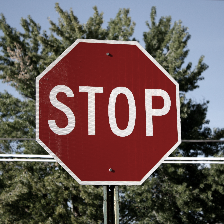
\includegraphics[width=0.2\linewidth]{../test_images/perturbed/stop_grayscale_0_500.png} & 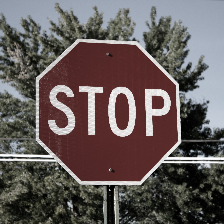
\includegraphics[width=0.2\linewidth]{../test_images/perturbed/stop_grayscale_0_250.png} & 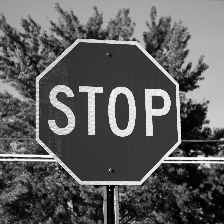
\includegraphics[width=0.2\linewidth]{../test_images/perturbed/stop_grayscale_0_010.png} \\
    \makecell{YOLOv3 = 0.99987 \\ RCNN = 0.99987} & \makecell{YOLOv3 = 0.99988 \\ RCNN = 0.99987} & \makecell{YOLOv3 = 0.99989 \\ RCNN = 0.99986} & \makecell{YOLOv3 = 0.99986 \\ RCNN = 0.99868} \\[1cm]
    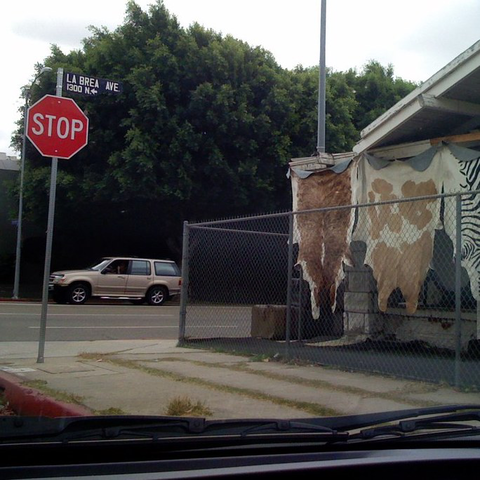
\includegraphics[width=0.2\linewidth]{../test_images/stop3.png} & 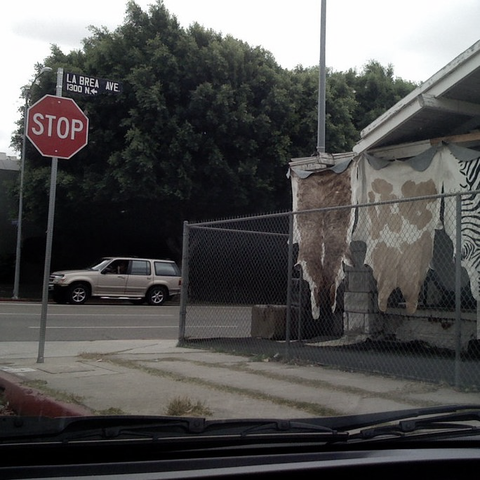
\includegraphics[width=0.2\linewidth]{../test_images/perturbed//stop3_grayscale_0_500.png} & 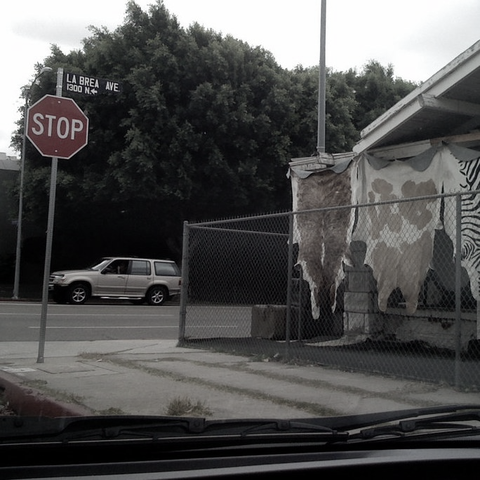
\includegraphics[width=0.2\linewidth]{../test_images/perturbed/stop3_grayscale_0_250.png} & 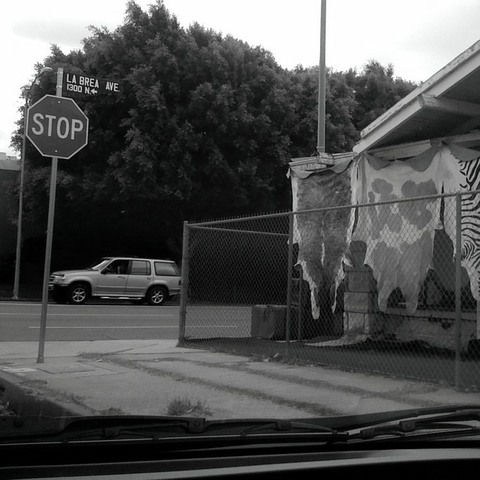
\includegraphics[width=0.2\linewidth]{../test_images/perturbed/stop3_grayscale_0_010.png} \\
    \makecell{YOLOv3 = 0.99971 \\ RCNN = 0.99839} & \makecell{YOLOv3 = 0.99971 \\ RCNN = 0.99859} & \makecell{YOLOv3 = 0.99970 \\ RCNN = 0.99866} & \makecell{YOLOv3 = 0.99965 \\ RCNN = 0.99846} \\  
\end{tabular}
\end{center}

\subsection{Contrast}
The contrast was adjusted for each of the images using the "Contrast" enhancer in Pillow's ImageEnhance package. The contrast parameter given to this enhancer is shown at the top of each column.
\begin{center}
\begin{tabular}{ c c c c }
    original & contrast = 0.05 & contrast = 0.025 & contrast = 0.01 \\
    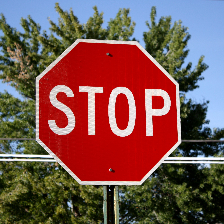
\includegraphics[width=0.2\linewidth]{../test_images/stop.png} & 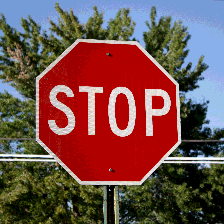
\includegraphics[width=0.2\linewidth]{../test_images/perturbed/stop_contrast_0_050.png} & 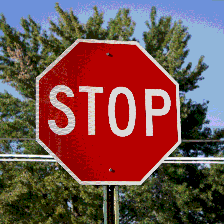
\includegraphics[width=0.2\linewidth]{../test_images/perturbed/stop_contrast_0_025.png} & 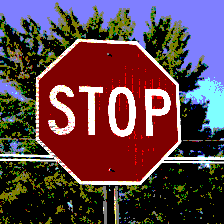
\includegraphics[width=0.2\linewidth]{../test_images/perturbed/stop_contrast_0_010.png} \\
    \makecell{YOLOv3 = 0.99987 \\ RCNN = 0.99987} & \makecell{YOLOv3 = 0.99985 \\ RCNN = 0.99994} & \makecell{YOLOv3 = 0.99986 \\ RCNN = 0.99993} & \makecell{YOLOv3 = 0.99984 \\ RCNN = 0.99859} \\[1cm]
    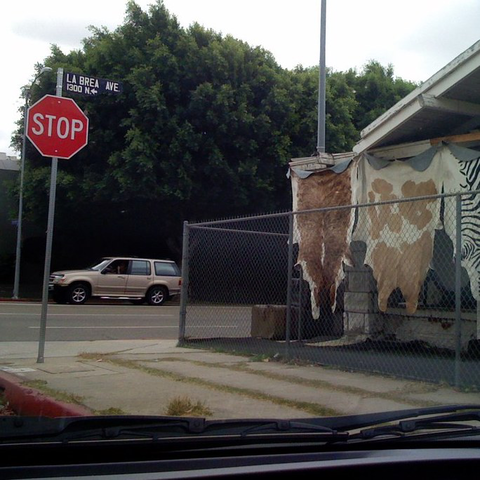
\includegraphics[width=0.2\linewidth]{../test_images/stop3.png} & 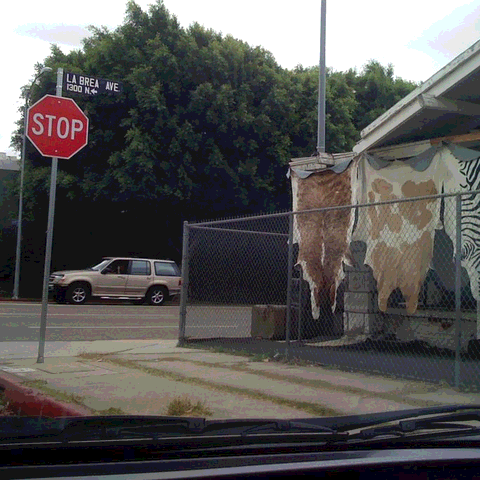
\includegraphics[width=0.2\linewidth]{../test_images/perturbed/stop3_contrast_0_050.png} & 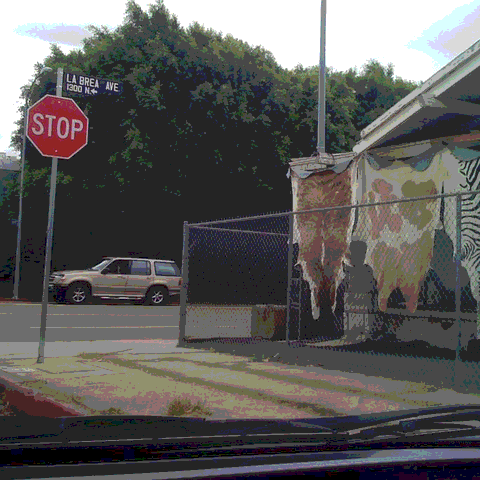
\includegraphics[width=0.2\linewidth]{../test_images/perturbed/stop3_contrast_0_025.png} & 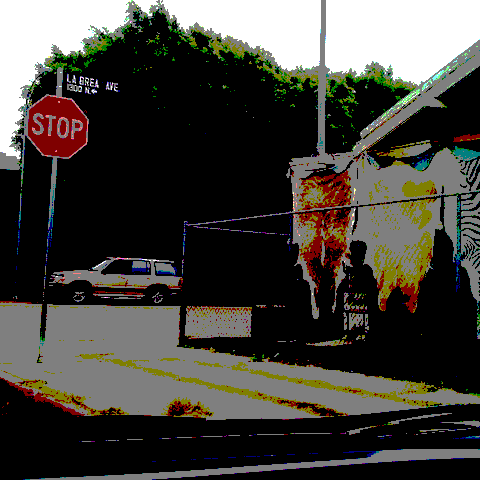
\includegraphics[width=0.2\linewidth]{../test_images/perturbed/stop3_contrast_0_010.png} \\
    \makecell{YOLOv3 = 0.99971 \\ RCNN = 0.99839} & \makecell{YOLOv3 = 0.99961 \\ RCNN = 0.99849} & \makecell{YOLOv3 = 0.99960 \\ RCNN = 0.99830} & \makecell{YOLOv3 = 0.99990 \\ RCNN = 0.99893} \\  
\end{tabular}
\end{center}

\subsection{Multiple Perturbations}
For these images all 3 perturbations were applied. First the contrast was set to 0.025, then noise was added with a multiplier of 200, and finally the color was removed from the image. 
\begin{center}
\begin{tabular}{ c c }
    original & perturbed \\
    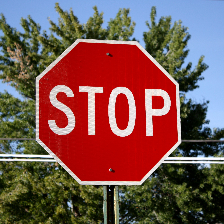
\includegraphics[width=0.4\linewidth]{../test_images/stop.png} & 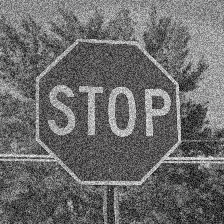
\includegraphics[width=0.4\linewidth]{../test_images/perturbed/stop_contrast_0_025_noise_200_grayscale_0_010.png} \\
    \makecell{YOLOv3 = 0.99987 \\ RCNN = 0.99987} & \makecell{YOLOv3 = 0.99992 \\ RCNN = 0} \\[1cm]
    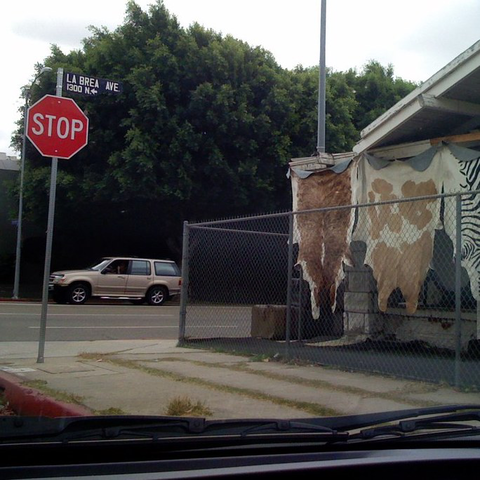
\includegraphics[width=0.4\linewidth]{../test_images/stop3.png} & 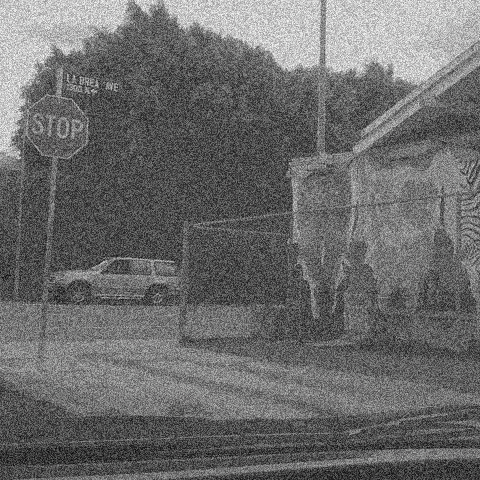
\includegraphics[width=0.4\linewidth]{../test_images/perturbed/stop3_contrast_0_025_noise_200_grayscale_0_010.png} \\
    \makecell{YOLOv3 = 0.99971 \\ RCNN = 0.99839} & \makecell{YOLOv3 = 0.99984 \\ RCNN = 0.99803} \\
\end{tabular}
\end{center}

As shown above random perturbation of images has little affect on the confidence score for both YOLOv3 and Faster-RCNN. The confidence score only drops when there is so much perturbation that it is difficult to see what it is as a human.

\section{Fast Gradient Sign Adversarial Images}

The fast gradient sign method for creating adversarial examples was first introduced by Goodfellow et al in \cite{goodfellow2015explaining}. This method works by computing the loss function for the input image, and then taking the derivative of the loss with respect to the input image. The sign of the gradient is then added to the input image to ascend the loss function and create as much misclassification error as possible.

\begin{equation}
    \eta = \epsilon * \text{sign} (\nabla_x L(x))
\end{equation}

Where $x$ is the input image, $L$ is the loss function which contains the classification model, $\epsilon$ is the learning rate, and $\eta$ is the perturbation to add to the input image.

The only problem with this method is that the output class that the model predicts after the perturbation is random, there isn't a way to choose it. A slight modification to the method was made so that instead of attempting to maximize the overall loss, the confidence score of a single class is used as the loss function to maximize. By optimizing this function, the confidence score of the target class will be increased.

\begin{equation}
    \eta = \epsilon * \text{sign} (\nabla_x (f_c(x))^2)
\end{equation}

Where $x$ is the input image and $f_c$ is the confidence score of the target class $c$ output by the model. This method was used to create adversarial examples on the VGG-16 \cite{simonyan2015deep} network, and run for several iterations until VGG-16 output the target class with a high confidence. Below is a comparison between the input image and the adversarial image that was created. The last column shows the difference between the 2 images scaled up so the differences are visible. The dark pixels changed the least and the lighter pixels changed the most.

\begin{center}
\begin{tabular}{ c c c }
    original & adversarial & difference \\
    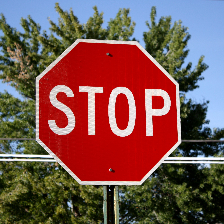
\includegraphics[width=0.3\linewidth]{../test_images/stop.png} & 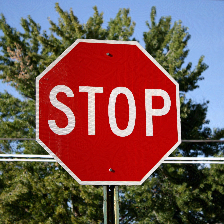
\includegraphics[width=0.3\linewidth]{../test_images/adversarial_vgg/stop.png} & 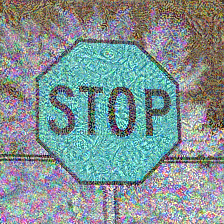
\includegraphics[width=0.3\linewidth]{../test_images/adversarial_vgg/stop_diff.png} \\
    \makecell{iPod confidence = 1.39 \\street sign confidence = 20.73} & \makecell{iPod confidence = 9.82 \\street sign confidence = 8.95} & \\
\end{tabular}
\end{center}

\section{Adversarial Examples Against YOLOv3}

\section{Ensemble Adversarial Examples}

\section{Dispersion Reduction}

\bibliographystyle{unsrt}
\bibliography{references}

\end{document}